\section{Results and discussion}\label{results_discussion}
Table \ref{raw_data1} presents the results of the experiments with the different algorithms on our data on Malaria. More specifically, Table \ref{raw_data1} contains the precision, the recall, the specificity, the AUC mesure, the score and F-measure of each algorithm tested while Figure 1 shows their respective ROC curve.  
\begin{table}[h]
\resizebox{\textwidth}{!}{
\centering
\scriptsize
{
\begin{tabular}{lccccccc}
\toprule
\cline{2-8}
 \textbf{ML ALgorithms} &  \textbf{Datasets} & \textbf{Precision} & \textbf{Recall} & \textbf{F1-score}&\textbf{AUC} &\textbf{Score}&\textbf{Specificity}\tabularnewline
\midrule
\cline{2-8}
 &  DT1 &0.97  & 1   & 0.98 & 0.78 & 97.04 & 0.05 \\
\cline{2-8}
& DT2 & 0.59 &0.48 &0.48  &0.64  &63.01  &0.80\\
\cline{2-8}
& DT3 &0.89  &0.85 &0.87  &0.86  &80.86  &0.69\\
\cline{2-8}
& DT4 &0.68  &0.57 &0.62  &0.70  &65.60  &0.74\\
\cline{2-8}
\multirow{-4}{*}{ \textbf{Decision Tree}}&   DT5 &0.99  &0.84 &0.91  &0.76  &83.41  &0.58\\
\midrule
\cline{2-8}
&DT1 &0.97 &1   &0.99 &0.81 &97.13& 0.07\\
\cline{2-8}
 & DT2 &0.63  & 0.34  &0.44&0.64&63.33& 0.85\\
 \cline{2-8}
 & DT3 &0.89 &0.85 &0.87&087&80.86&0.70\\
 \cline{2-8}
 & DT4 &0.68 &0.56&0.62&0.70&65.82&0.74\\
\cline{2-8}
\multirow{-4}{*}{ \textbf{Random Forest}}&   DT5 &0.99 &0.84&0.91&0.76&78.35&0.60\\
\midrule
\cline{2-8}
&DT1 &0.97 &1   &0.99 &0.79 &97.19&0.05 \\
\cline{2-8}
 &DT2 & 0.58 &0.36   &0.44&0.63&61.96&0.81\\
 \cline{2-8}
  &DT3 &0.85 &0.88 &0.86&0.86&79.59&0.55\\
  \cline{2-8}
  &DT4 &0.98 &0.56&0.92&0.70&65.82&0.72\\
  \cline{2-8}
\multirow{-4}{*}{ \textbf{Logistic Regression}}&   DT5 & 0.90&0.78&0.88&0.84&81.86&0.75\\
\bottomrule
\cline{2-8}
& DT1 &0.97 &1   &0.99 &0.81 &97.13 &0.00\\
 \cline{2-8}
  &DT2 & 0.60 &0.34   &0.43&0.63&62.86&0.83 \\
  \cline{2-8}
  &DT3 &0.86 &0.87 &0.86&0.85&79.94&0.60\\
  \cline{2-8}
  &DT4 &0.68 &0.59&0.63&0.70&65.63&0.73\\
  \cline{2-8}
\multirow{-4}{*}{ \textbf{Naive Bays}}&0.99 &0.82&0.90&0.84&85.61&0.71&0.71\\
\hline
\cline{2-8}
&DT1 &0.97 &1   &0.99 &0.84 &97.13&0.00 \\
\cline{2-8}
  &DT2 &0.58  &0.05   & 0.09&0.62&62.86&0.97\\
  \cline{2-8}
  &DT3 &0.57 & 0.86&0.86&0.85&79.94&0.64\\
  \cline{2-8}
 & DT4 & 0.68&0.58&0.62&0.70&65.63&0.73\\
 \cline{2-8}
 \multirow{-4}{*}{ \textbf{Support V Machine}}& DT5 &0.99 &0.86&0.92&0.80&85.61&0.62\\
 \hline
\cline{2-8}
&DT1 &0.97&1 &0.99   &0.84 &97.15&0.04  \\
\cline{2-8}
&  DT2 &0.59  &0.40   &0.48&0.65&62.86&0.80 \\
\cline{2-8}
 & DT3 &0.89 &0.85 &0.87&0.87&86.68&0.69\\
 \cline{2-8}
 & DT4 &0.68 &0.58&0.62&0.70&0.70&0.75\\
  \cline{2-8}
  \multirow{-4}{*}{ \textbf{ Artificial N Network}}&DT5 &0.99 &0.84&0.91&0.79&83.26&0.65\\ 
  \hline
\end{tabular}
}
}
\caption{Performances measures of our classifiers over all datasets}\label{raw_data1}
\end{table}
%
\begin{figure}[h]
\resizebox{\textwidth}{!}{
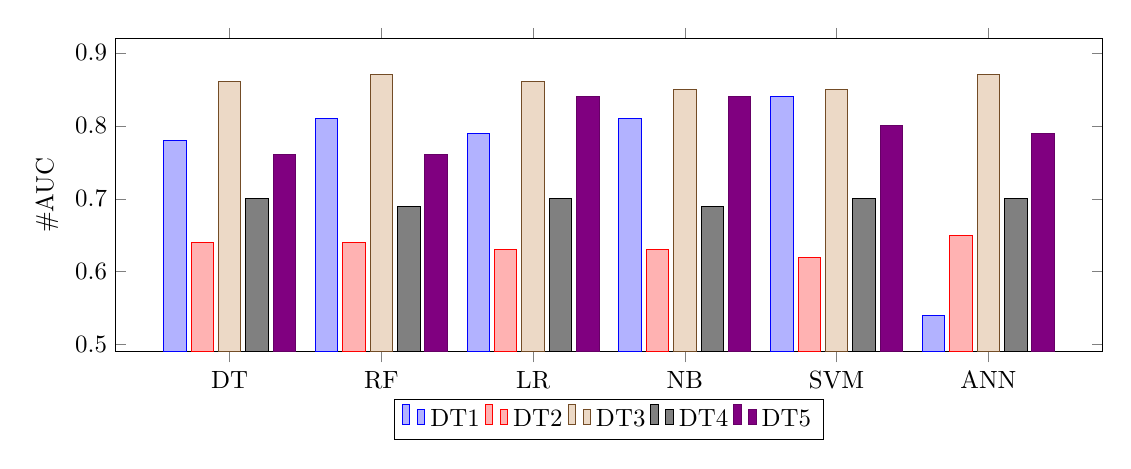
\begin{tikzpicture}[scale=0.9]
 \centering
\begin{axis}[
    height=6cm, width=15.5cm,
    bar width=0.4cm,
    ybar,
    %ybar=5pt,% configures `bar shift'
    bar width=9pt,
    enlargelimits=0.15,
    legend style={at={(0.5,-0.15)},
    anchor=north,legend columns=-1},
    ylabel={\#AUC},
    symbolic x coords={{DT,RF,LR,NB,SVM,ANN}},
    xtick=data,
    %nodes near coords,
    nodes near coords align={vertical},
    ]
\addplot coordinates {(DT,0.78) (RF, 0.81) (LR,0.79)(NB, 0.81)(SVM,0.84)(ANN, 0.54)};
\addplot coordinates{(DT,0.64) (RF, 0.64) (LR,0.63)(NB, 0.63)(SVM,0.62)(ANN, 0.65)};
\addplot coordinates {(DT,0.86) (RF, 0.87) (LR,0.86)(NB, 0.85)(SVM,0.85)(ANN, 0.87)};
\addplot coordinates {(DT,0.70) (RF, 0.69) (LR,0.70)(NB, 0.69)(SVM,0.70)(ANN, 0.70)};
\addplot coordinates {(DT,0.76) (RF, 0.76) (LR,0.84)(NB, 0.84)(SVM,0.80)(ANN, 0.79)};
\legend{DT1,DT2,DT3,DT4,DT5}
\end{axis}
\end{tikzpicture}
}
\caption{Comparison of the ROC Curves of the classifiers on differents datasets}
\end{figure}
 Looking closely at the results in terms of precision, recall and F-measure we observe that the classifiers RF, LR, SVM and ANN generally outperform the others for each dataset. Indeed, for the dataset DT1, which contains observations on patients living in different regions of Senegal, these four classifiers have an accuracy of 99\%, a recall greater than 92\% and an F-measure greater than 95\%. We note the same trend with the DT2 dataset which contains observations on patients living in the same area in Senegal. It can also be noted that RF, LR, SVM and ANN have better precision than the rapid diagnostic test carried out and systematically used in the majority of health structures in Senegal. 

\begin{figure}[!h]
%\subfigure[Precision values of compared classifiers on different datasets]{
\resizebox{\textwidth}{!}{
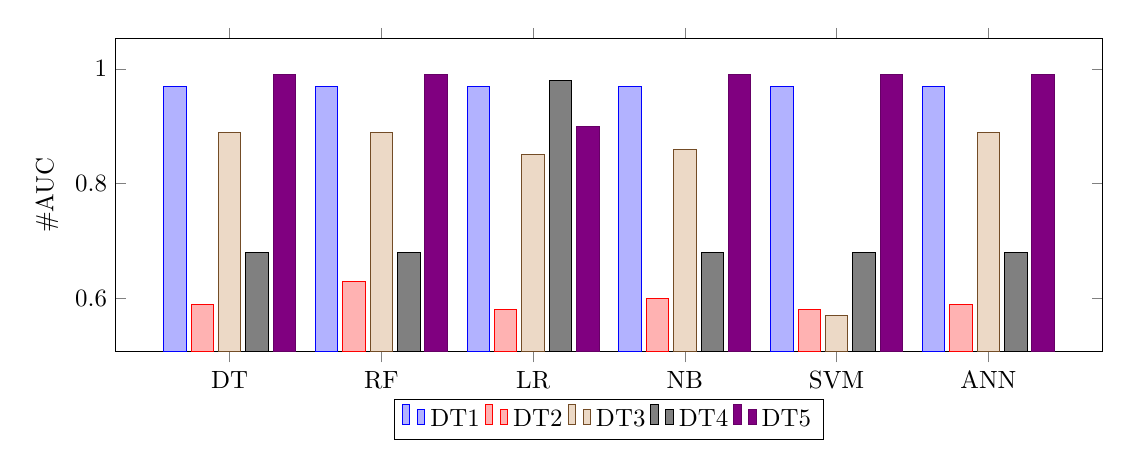
\begin{tikzpicture}[scale=0.9]
 %\centering
\begin{axis}[
     height=6cm, width=15.5cm,
    bar width=0.4cm,
    ybar,
    %ybar=5pt,% configures `bar shift'
    bar width=9pt,
    enlargelimits=0.15,
    legend style={at={(0.5,-0.15)},
    anchor=north,legend columns=-1},
    ylabel={\#AUC},
    symbolic x coords={{DT,RF,LR,NB,SVM,ANN}},
    xtick=data,
    %nodes near coords,
    nodes near coords align={vertical},
    ]
\addplot coordinates {(DT,0.97) (RF, 0.97) (LR,0.97)(NB, 0.97)(SVM,0.97)(ANN, 0.97)};
\addplot coordinates{(DT,0.59) (RF, 0.63) (LR,0.58)(NB, 0.60)(SVM,0.58)(ANN, 0.59)};
\addplot coordinates {(DT,0.89) (RF, 0.89) (LR,0.85)(NB, 0.86)(SVM,0.57)(ANN, 0.89)};
\addplot coordinates {(DT,0.68) (RF, 0.68) (LR,0.98)(NB, 0.68)(SVM,0.68)(ANN, 0.68)};
\addplot coordinates {(DT,0.99) (RF, 0.99) (LR,0.90)(NB, 0.99)(SVM,0.99)(ANN, 0.99)};
\legend{DT1,DT2,DT3,DT4,DT5}
\end{axis}
\end{tikzpicture}
}
\caption{Precision values of compared classifiers on different datasets}
\end{figure}


